\chapter[Nonlinear BVP]{A Tricky Nonlinear Boundary Value Problem}
The problem discussed today has been solved in Mark Holmes (1995) pp.69--73; the analysis here diverges from that in the book (so care needed)!

\paragraph{Example:} This \underline{nonlinear} BVP shows another kind of interior layer -- a \emph{shock layer} -- which is different from a \emph{corner layer} discussed in the previous lecture.
\begin{gather*}
	\epsilon y'' = \underline{yy'} - y\\
	y(0) = 1 \qquad y(1) = -1 \\
	\qquad 0 <x<1 \qquad \epsilon \rightarrow 0^+ 
\end{gather*}
\begin{itemize}
	\item In nonlinear problems, linear superpositions of solutions are not necessarily solutions anymore.
	\item Unlike in the linear case, there is no theory that tells us where layers are. So one approach is to try layers at $x=0$, $x=1$ or $x=x_0$ and try to match the solutions like usual. However, in nonlinear problems there may be multiple layers! Plus this could be a lot of work...
\end{itemize}
The approach here is to perform a \emph{phase plane analysis}. Regard $x$ as time $t$ and introduce a new variable $z=y'$ which yields the coupled equation
	\begin{align*}
	y' &= z \\
	z' &= \frac{1}{\epsilon} y(z-1)
	\end{align*}
on the $(y,z)$ phase-plane. So at every point $(y,z)$, there is a corresponding ``velocity'' vector-field $(y',z')$ which tells us which direction to move in at that instantaneous time/point.
\begin{figure}[!h]
	\centering
	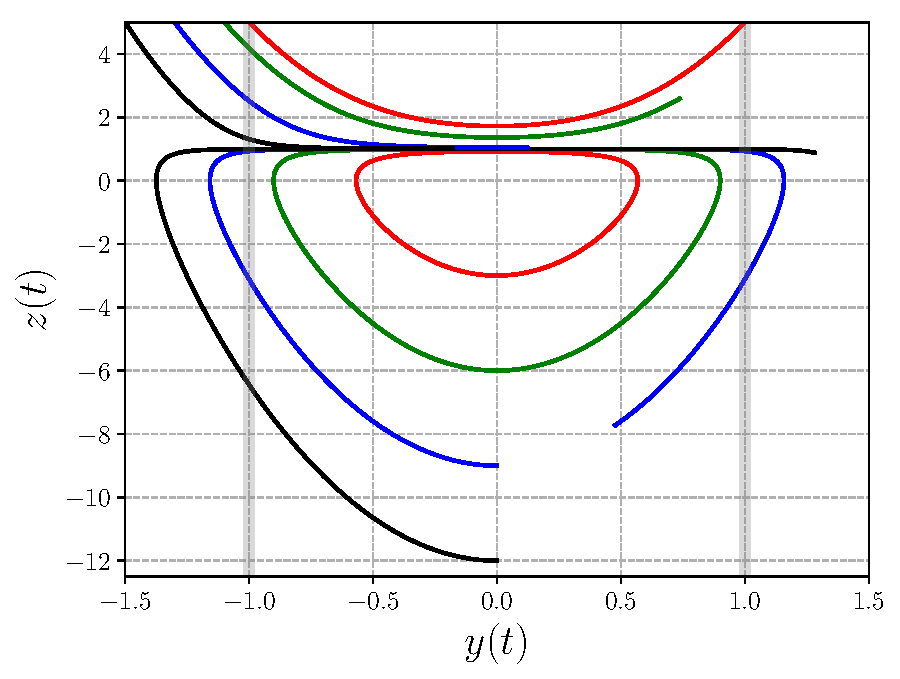
\includegraphics[width=0.65\textwidth]{./plots/pdf/strogatz-wk16.pdf}
	\caption{Here $\epsilon=0.1$. The vertical gray lines at $y(t) =\pm 1$ are the boundary values. The ``particles'' above $z=1$ were launched at $z=5$ while those below this line were launched at $y=0$. The ``open'' curves ($z>1$) are run for $t=1$; the ``closed'' curves ($z<1$) are run for $t=3$.}
	\label{fig:strogatz-wk16}
\end{figure}
Note the following:
\begin{itemize}
	\item The second order ODE is determined either by the boundary values ($y=\pm 1$) or initial values. The latter corresponds to specifying $(y,y') = (y,z)$ at $t=0$.  This is plotted in Fig. \ref{fig:strogatz-wk16} for a variety of ICs.
	\item For a chosen value (duration) of the parameter $t=t(x)=x$, the ``correct'' $y'$ is the value of $z(0)$ which satisfies the BC stipulated by our BVP.
	\item Alternatively, for each initial $z(0)$, we can always find a value of $t$ which will satisfy the left BC. But since $t=t(x)$ and $x \in (0,1)$ is prescribed, there is a ``correct'' $t=1$.
\end{itemize}
We can prove that all the trajectories that lie below the \emph{invariant} line $z=1$ are closed curves. Use symmetry in this particular system:
\begin{align*}
	y' &= z \\
	z' &= \frac{1}{\epsilon} y (z-1)
\end{align*}
{\color{red} My argument does not appear correct for $z<1$ and $z>1$.} Observe that if $z>1$, both $z$ and $z-1$ remain positive for all values of $z$ and under the transformation
\begin{align*}
	z &\rightarrow z \\
	x &\rightarrow -x \\
	y &\rightarrow -y
\end{align*}
the coupled ODE remains the same. In other words, if $(y(x),z(x))$ is a trajectory, so is $(-y(-x),z(-x))$. So as $x$ (equivalently time $t$) runs backwards, $z(-t)=z(t)$ remains unchanged whereas $y(-t) = -y(t)$, i.e. there is a reflection about $y=0$. The trajectories are therefore \emph{closed curves}. Such ODEs are called ``reversible''. However if $ z<1$, $z$ and $z-1$ can be $+/-$, breaking the symmetry and the curves are no longer closed. \\
\ \newline
So far we have not used the fact that $0 <\epsilon \ll 1$. Consider two case:
\begin{itemize}
	\item If $y \neq 0$ and $z-1 = O(1)$, i.e. we are not too close to that invariant line $z=1$, then $1/\epsilon \rightarrow \infty$ meaning that $z'=O(1/\epsilon) \gg y'$. So the vertical velocity is huge and the variation in $z$ is very rapid cf. $y$. This is the dynamical equivalent of a ``layer'' or \underline{inner} solution!
	\item Otherwise, if $z-1=O(\epsilon)$, then $y' \approx z'=O(1)$. This corresponds to the \underline{outer} solution.
\end{itemize}  
To know where the layer may occur, we can try launching a particle with different $y'(0)$ as shown in Fig. \ref{fig:strogatz-wk16-z-guess}. From Fig. \ref{fig:strogatz-wk16} the slope $y'(t)=z(t)$ peaks at $y=0$ and is therefore suggestive of an ``interior layer'' near $t=0.5$ if we pick the \emph{symmetric solution}. Note that other solutions are possible and this has been discussed in depth by \href{https://arxiv.org/abs/2107.11624}{Clark et al}. 
\begin{figure}[!h]
	\centering
	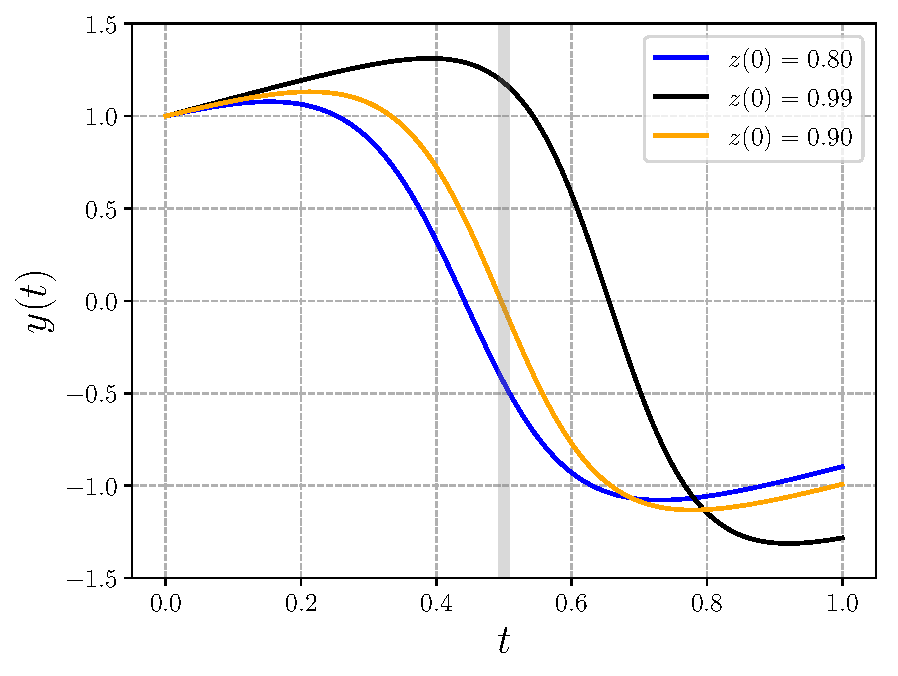
\includegraphics[width=0.65\textwidth]{./plots/pdf/strogatz-wk16-z-guess.pdf}
	\caption{We start with different launch angles close to $z=1$ to understand the presence of the layer.}
	\label{fig:strogatz-wk16-z-guess}
\end{figure}\\
We now revert to standard BL thinking and construct a solution of this type. The \underline{outer} solution is obtained by formally setting $\epsilon=0$. To the lowest order
\begin{gather*}
	y_0 y_0' - y_0 = 0
\end{gather*}
So either 
\begin{gather*}
	y_0 = 0 \qquad \text{or} \qquad  y_0 = x + a
\end{gather*}
Using the BCs
\begin{align*}
	y_0^L & = x+1 \\
	y_0^R & = x-2
\end{align*}
To deal with the \underline{inner} region, we define
\begin{gather*}
	X = \frac{x-1/2}{\delta}
\end{gather*}
yielding
\begin{align*}
	y' &= \frac{\md y}{\md X} \frac{\md X}{\md x} = \frac{1}{\delta} Y_X \\
	y'' &= \frac{1}{\delta^2} Y_{XX}
\end{align*}
where $y(x)=Y(X\delta + 1/2)$ together with the governing ODE
\begin{gather*}
	\epsilon \frac{1}{\delta^2} Y'' = Y\frac{1}{\delta}Y'-Y
\end{gather*}
From dominant balance
\begin{gather*}
	\frac{\epsilon}{\delta^2} \approx \frac{1}{\delta} \gg 1
\end{gather*}
yielding $\delta = \epsilon$ and the inner equation
\begin{gather*}
	Y'' = YY' - \epsilon Y
\end{gather*}
To the lowest order ignoring $O(\epsilon)$ terms
\begin{gather*}
	Y_0'' = Y_0 Y_0' 
\end{gather*}
which is integrated to derive
\begin{gather*}
	Y_0' = \frac{1}{2} Y_0^2 + A
\end{gather*}
i.e. the arcs in the phase-plane are parabolas to the lowest order. Observe that at $Y=0$ our intercept has to be negative, so for convenience we can set
\begin{gather*}
	A = \frac{1}{2} b^2
\end{gather*}
This yields
\begin{gather*}
	\frac{\md Y_0}{Y_0^2 - b^2} = \frac{1}{2}\md X
\end{gather*}
Note that \\
\begin{minipage}[c]{0.49\linewidth}\small
	\begin{gather*}
	|x|<1 \\
	\frac{\md}{\md x} (\tanh^{-1} x) = \frac{1}{1-x^2}
	\end{gather*}
\end{minipage} \qquad 
\begin{minipage}[c]{0.49\linewidth} \small
	\begin{gather*}
	|x|>1 \\
	\frac{\md}{\md x} (\coth^{-1} x) = \frac{1}{1-x^2}
	\end{gather*}
\end{minipage} \\
\ \newline 
\ \newline 
This allows us to integrate to write
\begin{gather*}
	Y_0(X) = b \tanh \left(c - \frac{b}{2}X\right)
\end{gather*}
Noting that $Y_0(X=0)=0$ (from symmetry of this solution), we see $c=0$. Matching at the left boundary
\begin{align*}
	\lim\limits_{x \rightarrow 1/2} y^L_0(x) &= \lim\limits_{X \rightarrow -\infty} Y_0(X) \\
	\frac{3}{2} &= b
\end{align*} 
The right boundary matching condition also yields the same value for $b$. Collecting our solutions:
\begin{align*}
	y_0^L(x) &\sim x+1 \\
	y_0^R(x) &\sim x-2 \\
	Y(X) &\sim -\frac{3}{2} \tanh \left(\frac{3}{4}X\right)
\end{align*}
On the left half
\begin{align*}
	y_c &\sim y_0^L(x) + Y(X)_\text{inn} - y_\text{match} \\
	& \sim (x+1) -\frac{3}{2} \tanh \left[ \frac{3}{4}\left(\frac{x-1/2}{\epsilon}\right)\right] - \frac{3}{2}
\end{align*}
On the right half
\begin{align*}
y_c &\sim y_0^R(x) + Y(X)_\text{inn} - y_\text{match} \\
& \sim (x-2) -\frac{3}{2} \tanh \left[ \frac{3}{4}\left(\frac{x-1/2}{\epsilon}\right)\right] + \frac{3}{2}
\end{align*}
The two composite solutions are identical and the equation is odd about $x=1/2$. 



